\section{Analysing Trading Patterns}

\subsubsection{Presentation of Facts}

\subsection{Building the Robinhood Portfolio}
As explained above, the biggest limitation of the Robintrack dataset is that it counts the number of users holding a certain security and doesn't provide any information on the amount invested in a particular security. 

A possible solution is building a portfolio in which we assume that all positions hold the same equivalent amount of money in a certain security. This means weighing stocks by their "popularity":
\begin{equation*}
    Pop_{i,t}=\frac{n_{i,t}}{\sum_in_{i,t}}
\end{equation*}
where $n_{i,t}$ is the number of users holding a certain stock on a given day. This normalization is necessary to isolate the performance from the large influx of users on the platform.

We can therefore define the value of the  Robinhood Portfolio as follows:
\begin{equation*}
    V_{RH,t}=\sum_{i=1}^N Pop_{i,t}\cdot P_{i,t}
\end{equation*}

In comparison, the value of the reference index is simply the sum of the market cap for each security present in the Robinhood dataset. 

\subsection{Comparing Returns and Risk measures}
Having defined the value for the Robinhood Portfolio and reference index we can analyze their performance, also comparing them to the S\&P500 and a world ETF\footnote{VOO is the ticker of the Vanguard S\&P500 ETF} and VT is the ticker of Vanguard Total World Stock ETF) as general market proxies. 

Returns for a given time frame are computed as the sum of the daily log returns for the previous days.

Keeping this in mind we can obtain the moving average and cumulative returns for all these indices, as well as their distributions.

\begin{figure}[h!]
    \centering
    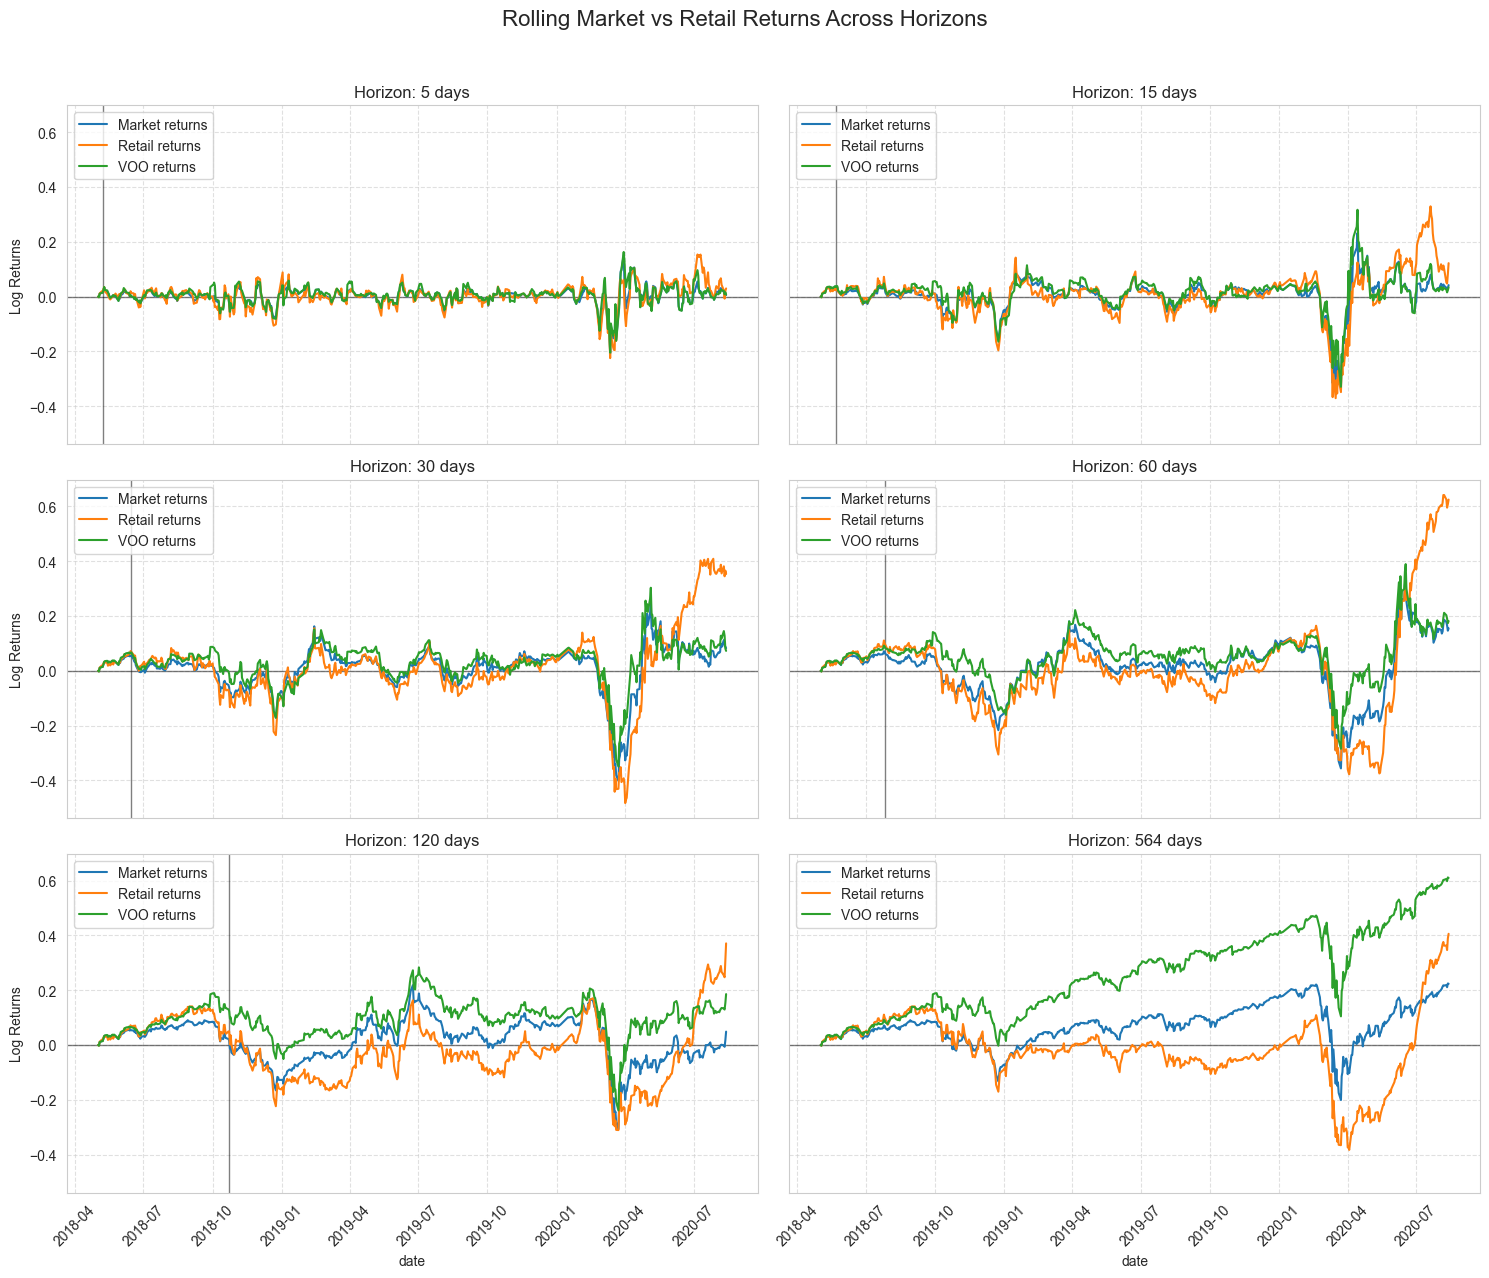
\includegraphics[width=1\linewidth]
    {Images/returns_comparison.png}
    \label{fig:enter-label}
\end{figure}

At short-term horizons (5 to 15 days), all three portfolios show similar patterns, with relatively mild fluctuations. Retail returns exhibit slightly higher volatility, particularly for the Robinhood portfolio, indicating that retail investors are more reactive to short-term market movements. The returns across these horizons reflect a degree of correlation, suggesting that, over short periods, retail investors' behavior mirrors that of the broader market, albeit with more pronounced movements.

At the 30- and 60-day horizons, divergence becomes more apparent. The Robinhood portfolio shows a higher degree of volatility, with both larger peaks and deeper troughs compared to the market and the ETF benchmarks (VOO and VT). This volatility suggests that retail traders may be engaging in more speculative behavior or reacting strongly to market news, which could lead to exaggerated responses and momentum chasing. Notably, during periods of rapid market movements (e.g., mid-2020), the Robinhood portfolio experiences sharp rallies, likely driven by retail investor participation in tech stocks or speculative assets.

At the 120-day horizon, the Robinhood portfolio begins to underperform relative to both VOO and VT, particularly in major market downturns like the COVID-19 crash. The underperformance during these periods is consistent with the behavior observed in retail investors during market corrections—often driven by overreaction or poor risk management. However, after the COVID market crash, the Robinhood portfolio shows notable recovery, achieving higher returns than VOO and VT, reflecting retail traders' ability to capitalize on post-crash rebounds, potentially due to increased exposure to riskier assets.

At the 564-day horizon, the long-term performance diverges significantly. The Robinhood portfolio initially lags behind both VOO and the market, reflecting a less optimal asset allocation or suboptimal stock selection. While there is some recovery post-COVID, retail investors still fail to capture the consistent growth observed in the broader market over a longer timeframe. This highlights the challenges that retail investors may face in achieving long-term growth, especially when influenced by short-term market sentiment or reacting to news-driven volatility. Nonetheless, the post-crash rally showcases the potential for retail portfolios to outperform during certain market phases, albeit with higher risk.

Overall, the plot demonstrates that while retail portfolios can experience significant short-term gains, their performance is often more volatile and less consistent over the medium to long term, with periods of underperformance and delayed recoveries.

Looking at the distribution of returns for the same periods other insights can be drawn (compare \ref{tab:returns_stats}). 

\begin{figure}[h!]
    \centering
    \includegraphics[width=1\linewidth]{Images/distributions_comparison.png}
\end{figure}

At shorter horizons (5 to 30 days), the return distributions for all portfolios- market, Robinhood (RH), VOO, and VT- are quite similar, with tightly clustered and symmetric shapes. However, the Robinhood distribution exhibits slightly fatter tails compared to VOO and the market, suggesting that retail investors, particularly those in the Robinhood portfolio, experience more extreme short-term gains and losses. This indicates higher short-term volatility and sensitivity to market movements.

As the horizon increases (60 to 564 days), the Robinhood distribution becomes increasingly dispersed, with wider tails and lower peaks. This shift indicates that retail investors are exposed to higher volatility over longer periods, with greater potential for both positive and negative extreme outcomes. In contrast, VOO and the market distributions remain relatively stable, with tighter and more concentrated peaks. These distributions suggest that diversified portfolios, like VOO and the market index, provide more consistent and lower-risk returns over time.

At the longest horizon (564 days), the Robinhood distribution shows a noticeable left skew, indicating that the portfolio underperforms over the long term. This is consistent with earlier findings of long-term underperformance, where retail investors fail to capture consistent gains in the broader market. In contrast, the VOO distribution is shifted rightward, reflecting stronger and more consistent long-term performance, which is typical of diversified, lower-risk portfolios.

In summary, these distribution plots highlight the increased volatility and higher risk exposure associated with the Robinhood portfolio, especially as the time horizon lengthens. Over both medium and long horizons, retail portfolios are more prone to extreme outcomes, with consistent underperformance relative to the more diversified VOO and market portfolios. This reinforces the conclusion that retail investors, while potentially benefiting from short-term rallies, struggle to maintain consistent returns in the long run due to greater sensitivity to market fluctuations and suboptimal asset selection.
\paragraph{What Happened during the Pandemic?} Analyzing the same indices from February 3rd, 2020 we can find some relevant insights. 

\begin{figure}[h]
    \centering
    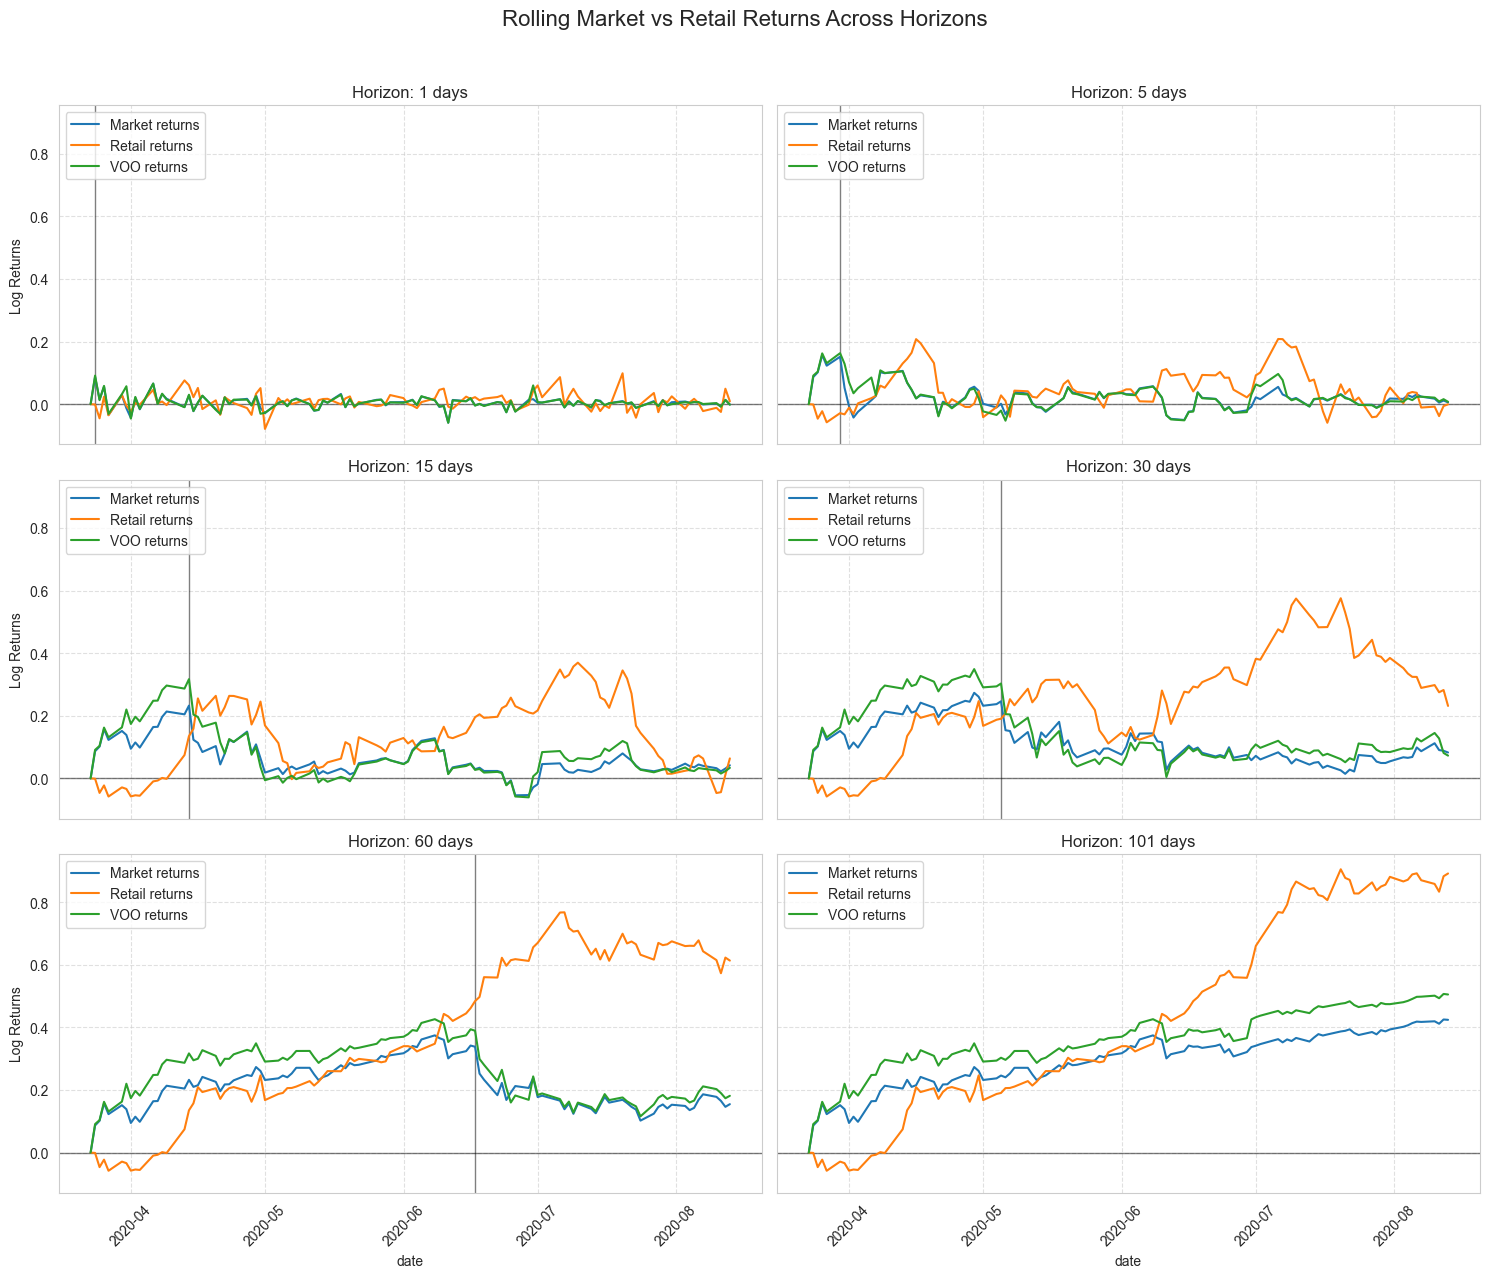
\includegraphics[width=1\linewidth]{Images/returns_comparison_pandemic.png}
\end{figure}
At very short horizons (1-5 days), performance across all portfolios is similar and volatile, with no consistent pattern. However, from the 15-day horizon onward, a clear divergence emerges: Robinhood portfolio returns (orange) begin to outpace both the market indices, which have a high degree of correlation.

This trend becomes particularly evident at 30, 60, and 135-day horizons, where the Robinhood portfolio exhibits significantly higher cumulative gains after a more sluggish start. 
In contrast, VOO and the market index recover more gradually, with smoother return paths and lower cumulative gains. This reflects broader diversification and reduced exposure to speculative stocks.

We can look at the distributions of returns for this timeframe as well:
\begin{figure}[H]
    \centering
    \includegraphics[width=1\linewidth]{Images/distributions_comparison_pandemic.png}
\end{figure}

\subsection{Analysis of Short-Term Market Movements and Volatility, Including the Impact of COVID}

\subsubsection{Return Characteristics and Volatility Analysis}
\paragraph{including COVID}
Comparing the daily and 5-day moving average returns for the whole period available we observe really similar behavior in terms of returns and distributions for the marker indices,
while RH has significantly fatter tails (which can be observed also in the CDF plot).

RH has slightly higher average returns compared to the market (MC) both for 1-day and 5-day returns. For 1-day returns, RH has an average return of 0.000719, which is higher than the market's 0.000396. 
Similarly, for 5-day returns, RH's average is 0.003281, which is again  higher than the market's 0.001913. 
In terms of standard deviation, RH shows more volatility in both horizons. 
The 1-day standard deviation for RH is 0.018809, compared to the market's 0.01547, and for the 5-day returns, RH's standard deviation is 0.041909, while the market's is 0.031198. 
Therefore, RH consistently exhibits higher returns and higher volatility over both timeframes compared to the market. Detailed distribution are in table \ref{tab:st_returns_stats_all}.

Here below the plots of the time series:
\begin{figure}[H]
    \centering
    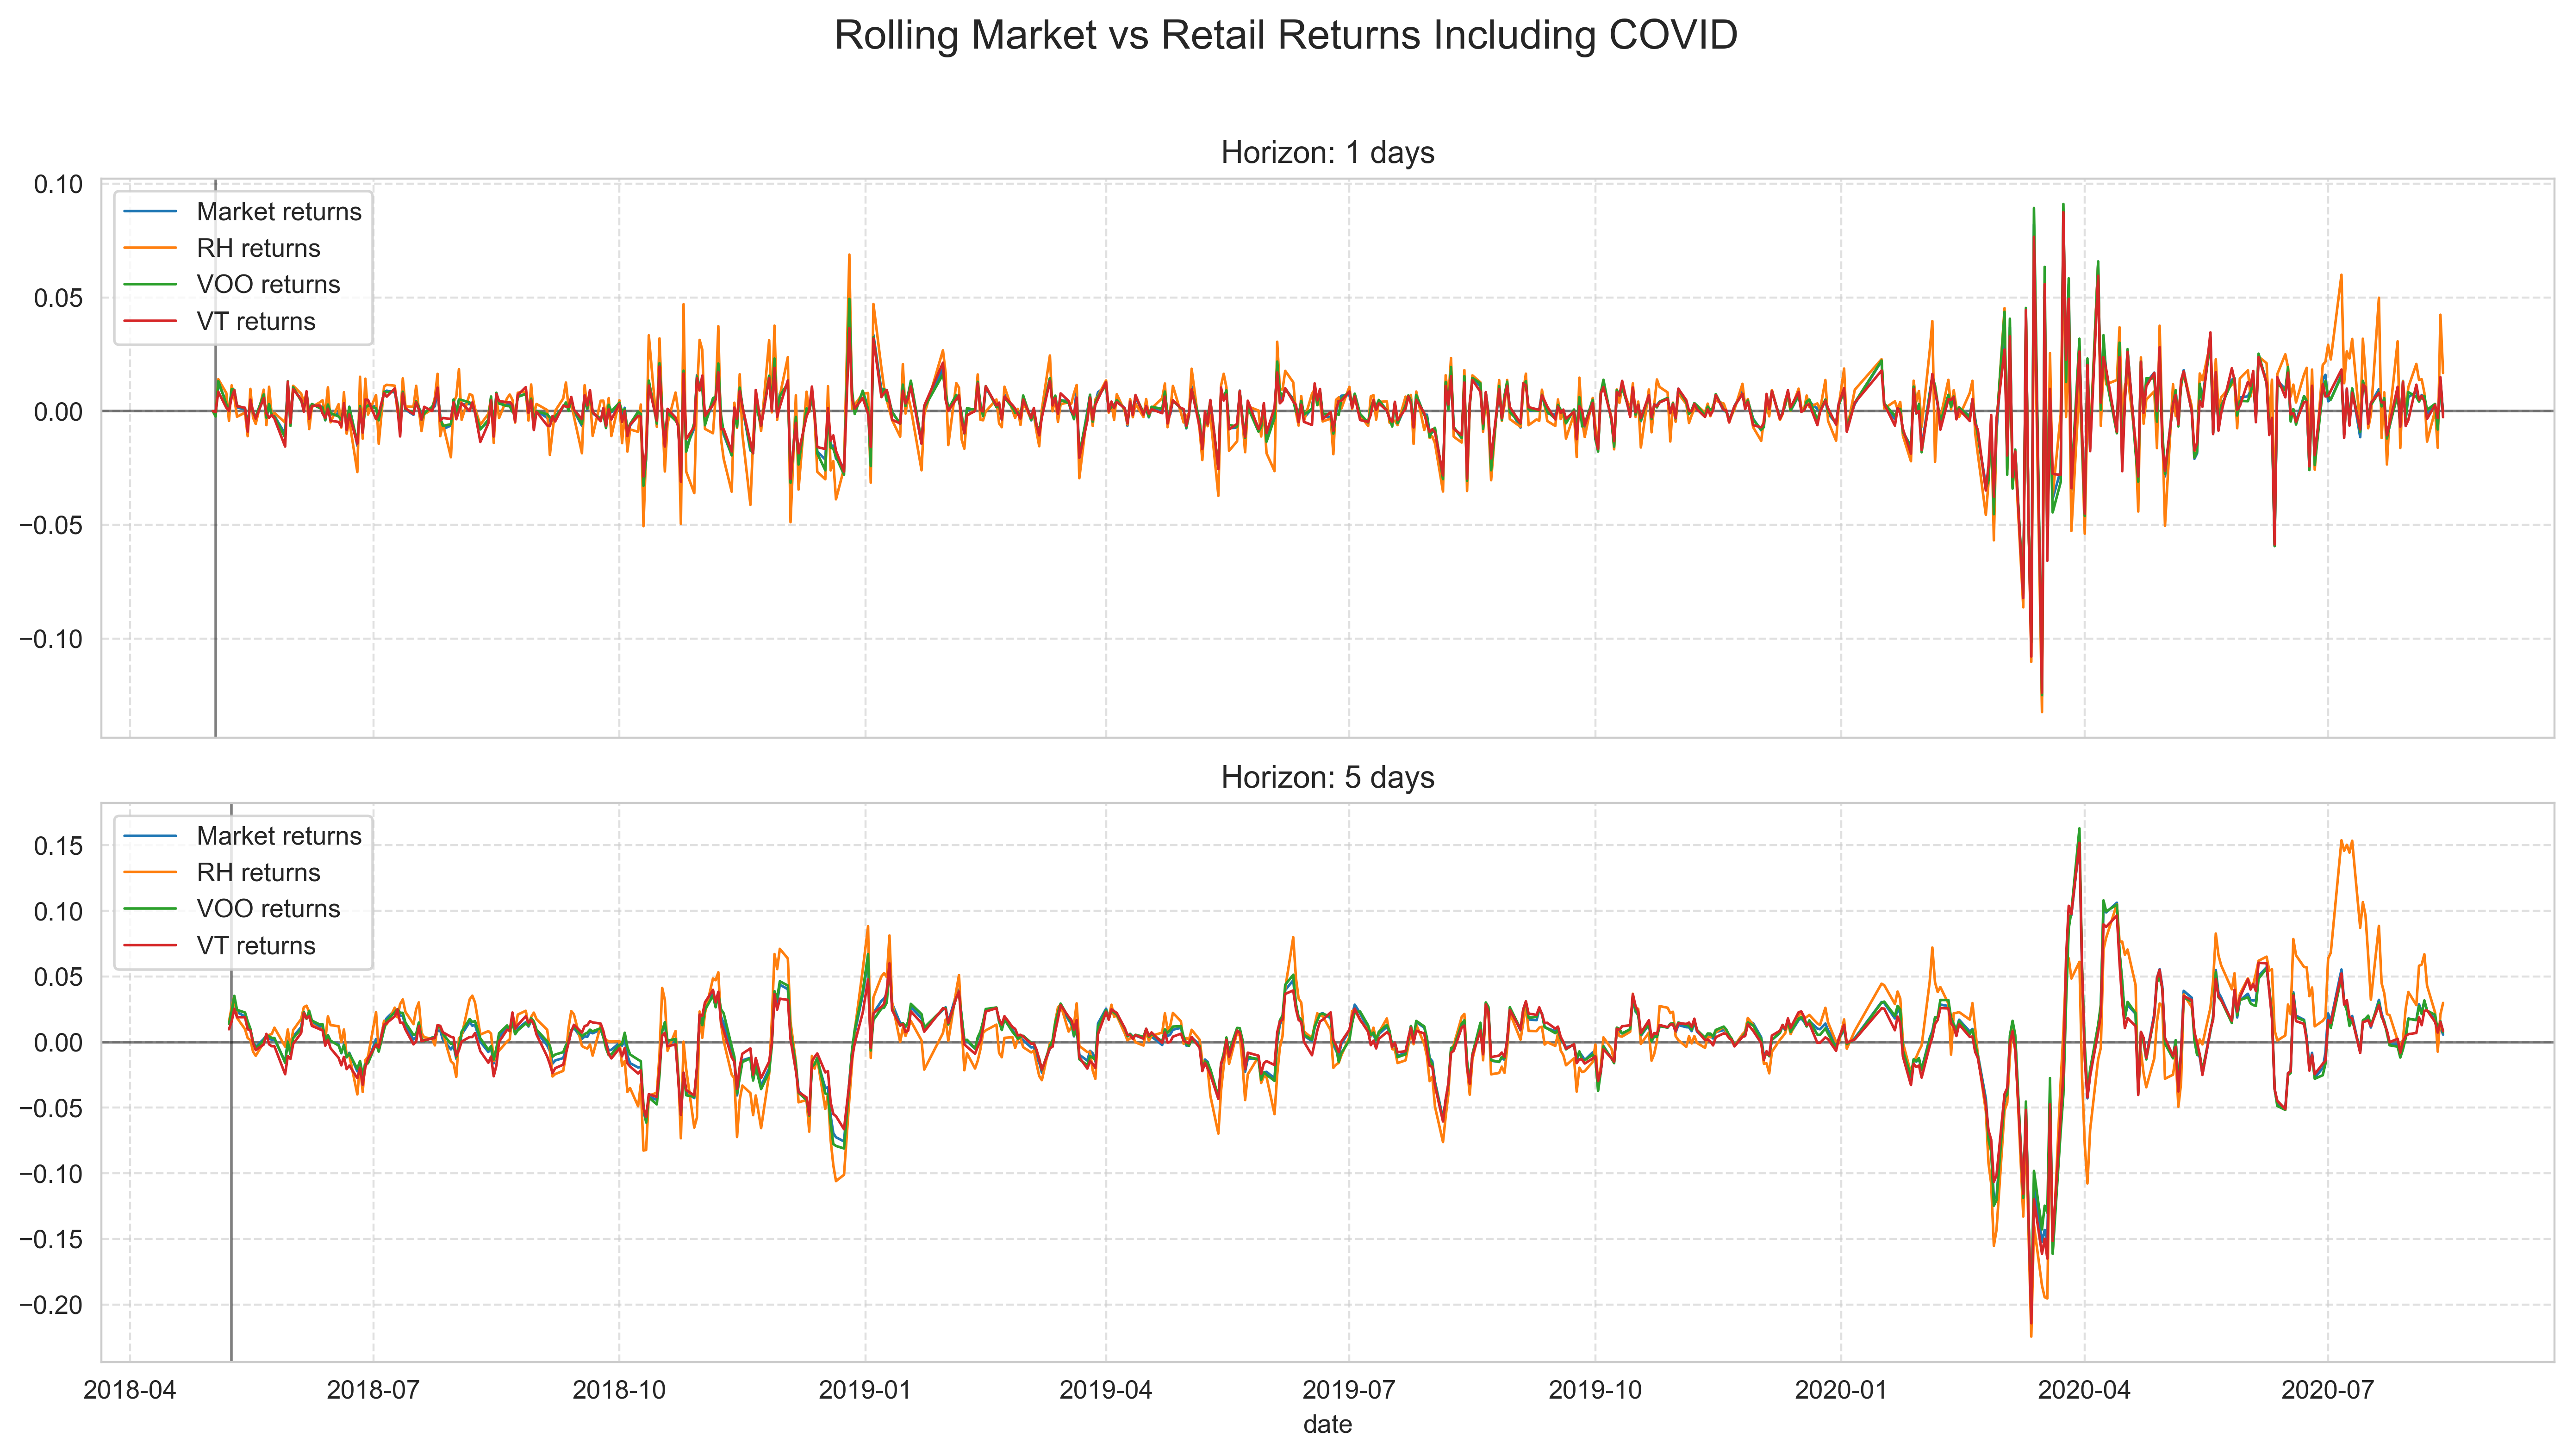
\includegraphics[width=1\linewidth]{Images/ts_including_1_5.png}
\end{figure}


\paragraph{Before COVID}
Excluding returns from February 3rd 2020 might help to reduce some of the noise in the sample and allow us to understand more significant trends about RH investors.

For 1-day returns, RH still has lower average returns compared to the market (MC). 
RH has an average return of 0.000115, while the market's average is 0.000419.

For the 5-day returns, RH's average is much smaller than that of the market. 
RH has an average return of 0.000259, while the market's average is 0.002091. 

In terms of standard deviation, RH still exhibits more volatility than the market, but the gap is again smaller than the previous data.
The 1-day standard deviation for RH is 0.013490, compared to 0.008745 for the market, which shows more volatility for RH but with a smaller gap compared to the earlier dataset where RH had much higher volatility.
For the 5-day standard deviation, RH has 0.026549, compared to 0.019395 for the market. The difference is still significant, but once again, smaller than the previous dataset where RH showed greater variability.

In conclusion, while RH still exhibits more volatility than the market across both horizons, it now shows lower returns than the market for both 1-day and 5-day periods, possibly due to a more consistent left tail.
Detailed distribution are in table \ref{tab:st_returns_stats_before}.

Here below the plots of the CDFs and PDFs, both including and exluding covid:
\begin{figure}[H]
    \centering
    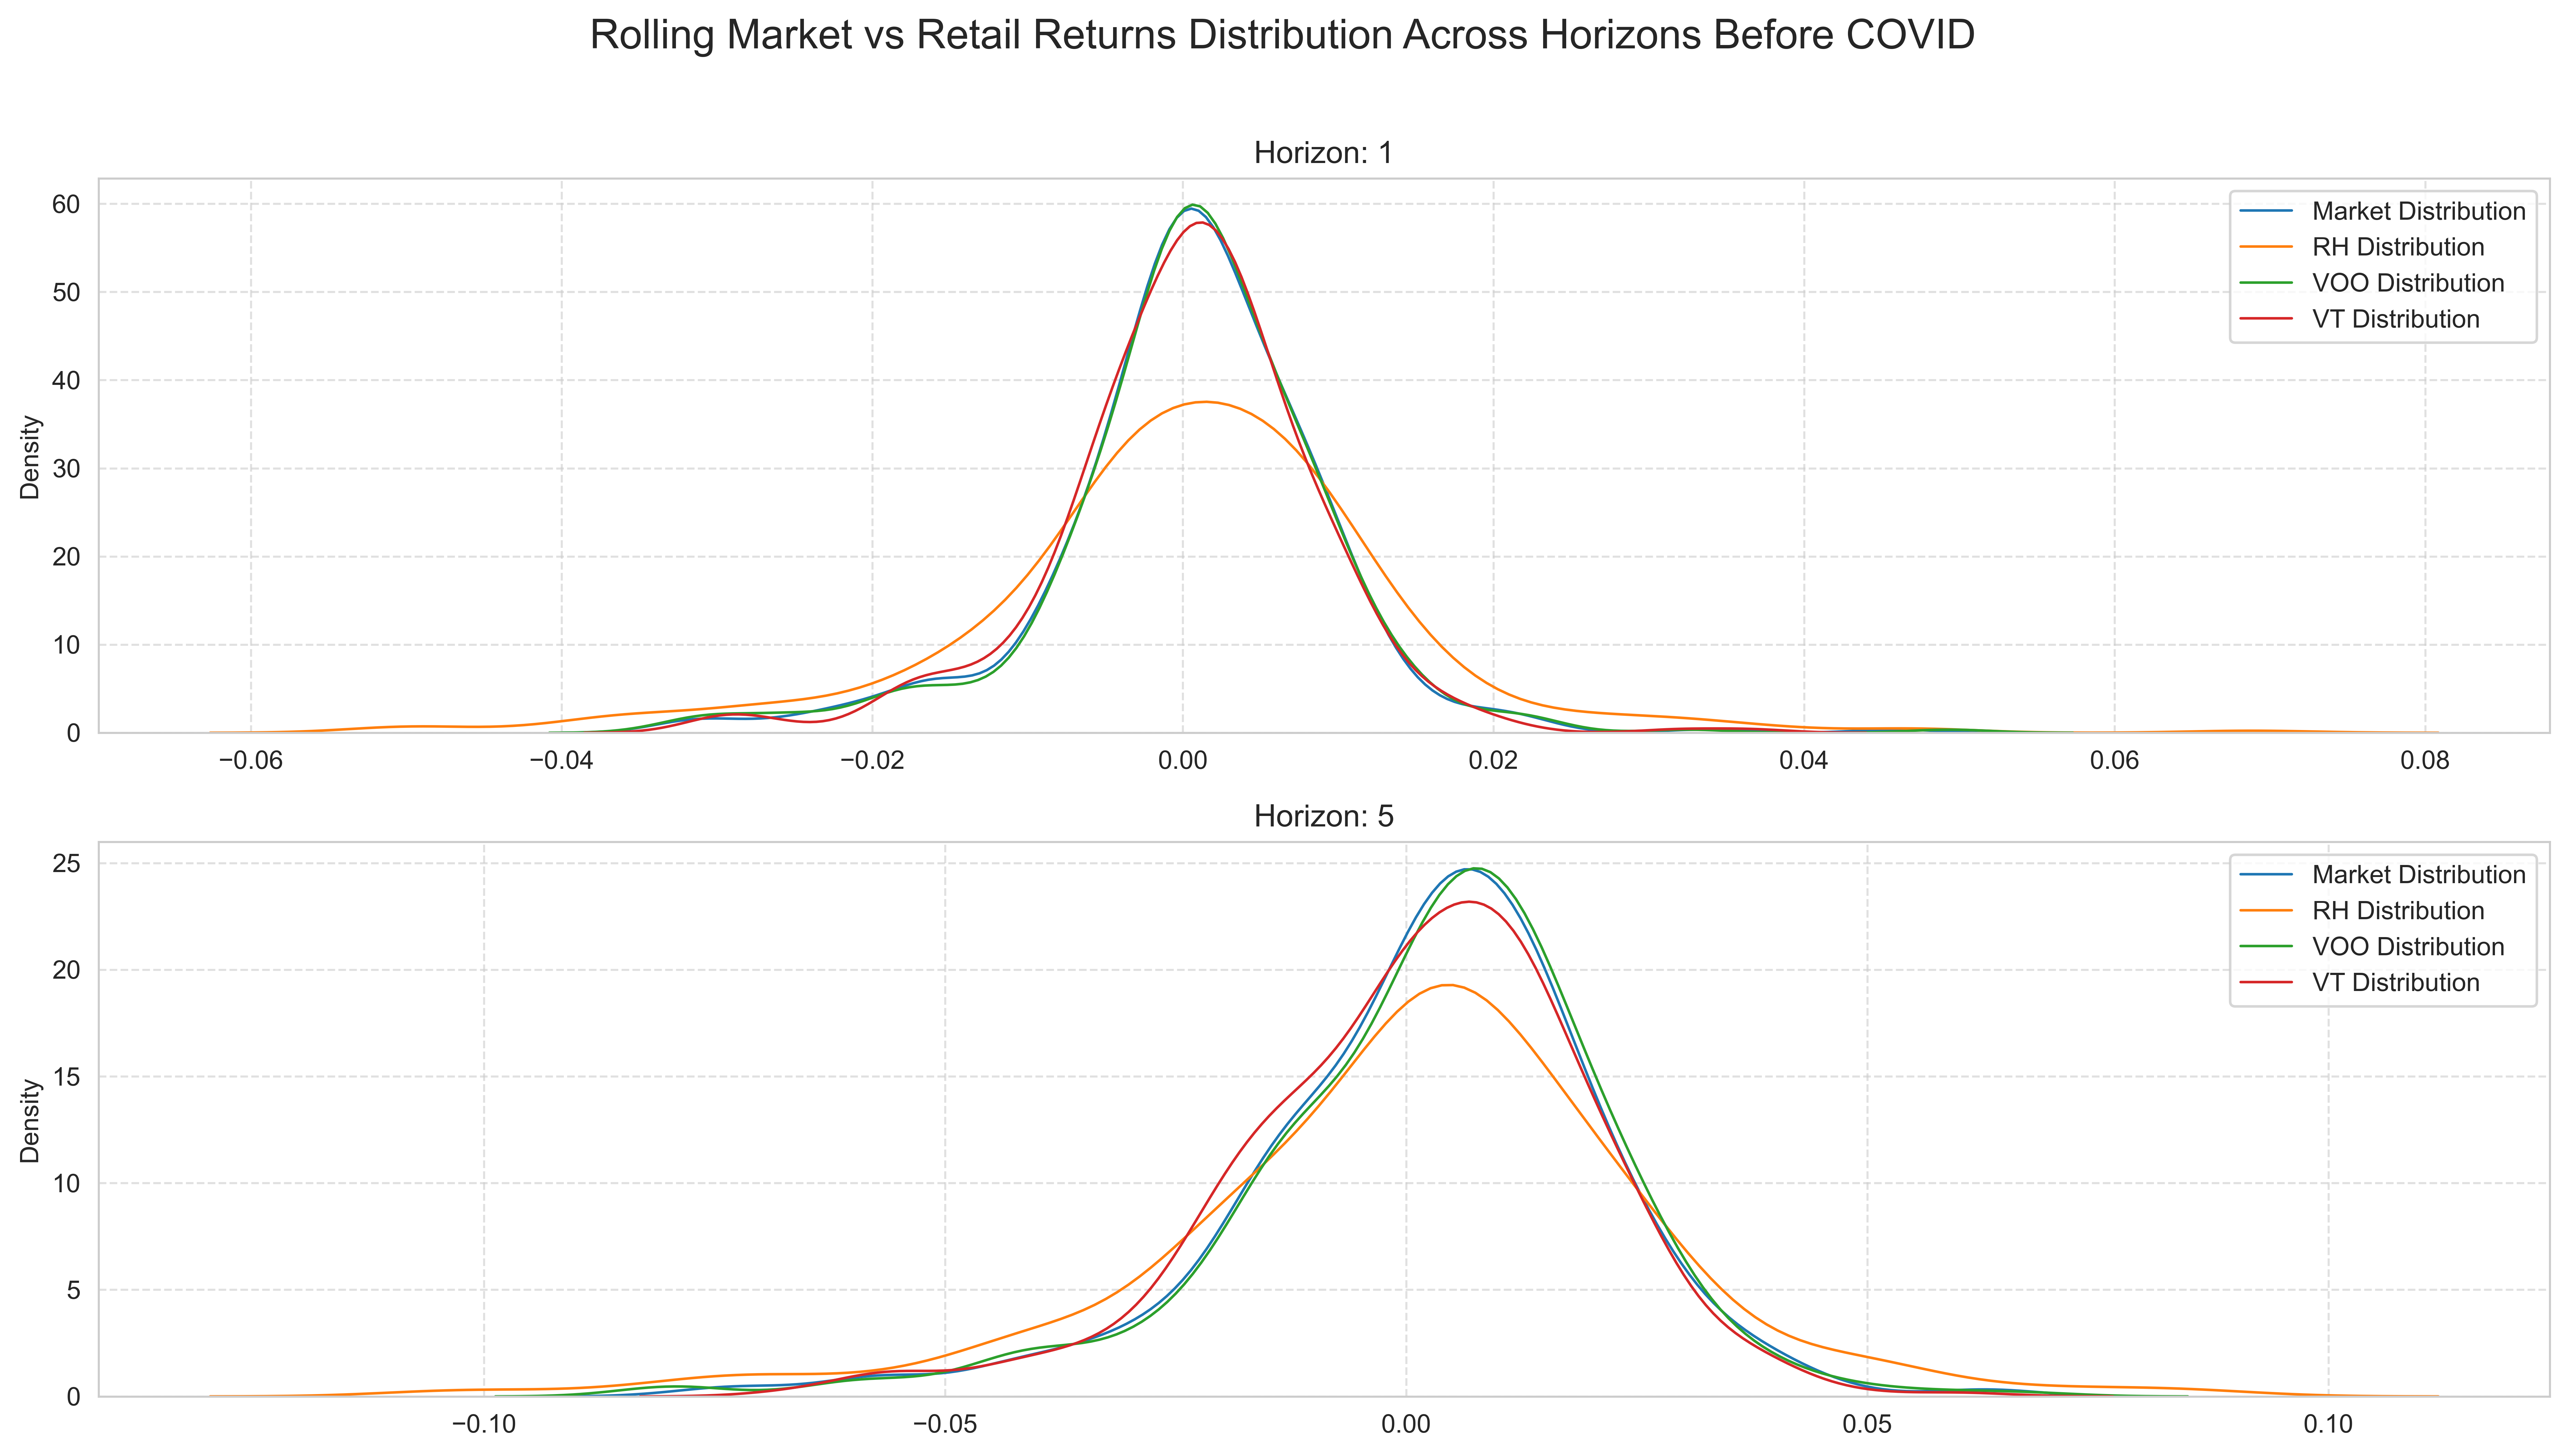
\includegraphics[width=1\linewidth]{Images/kdes_before_1_5.png}
\end{figure}
\begin{figure}[H]
    \centering
    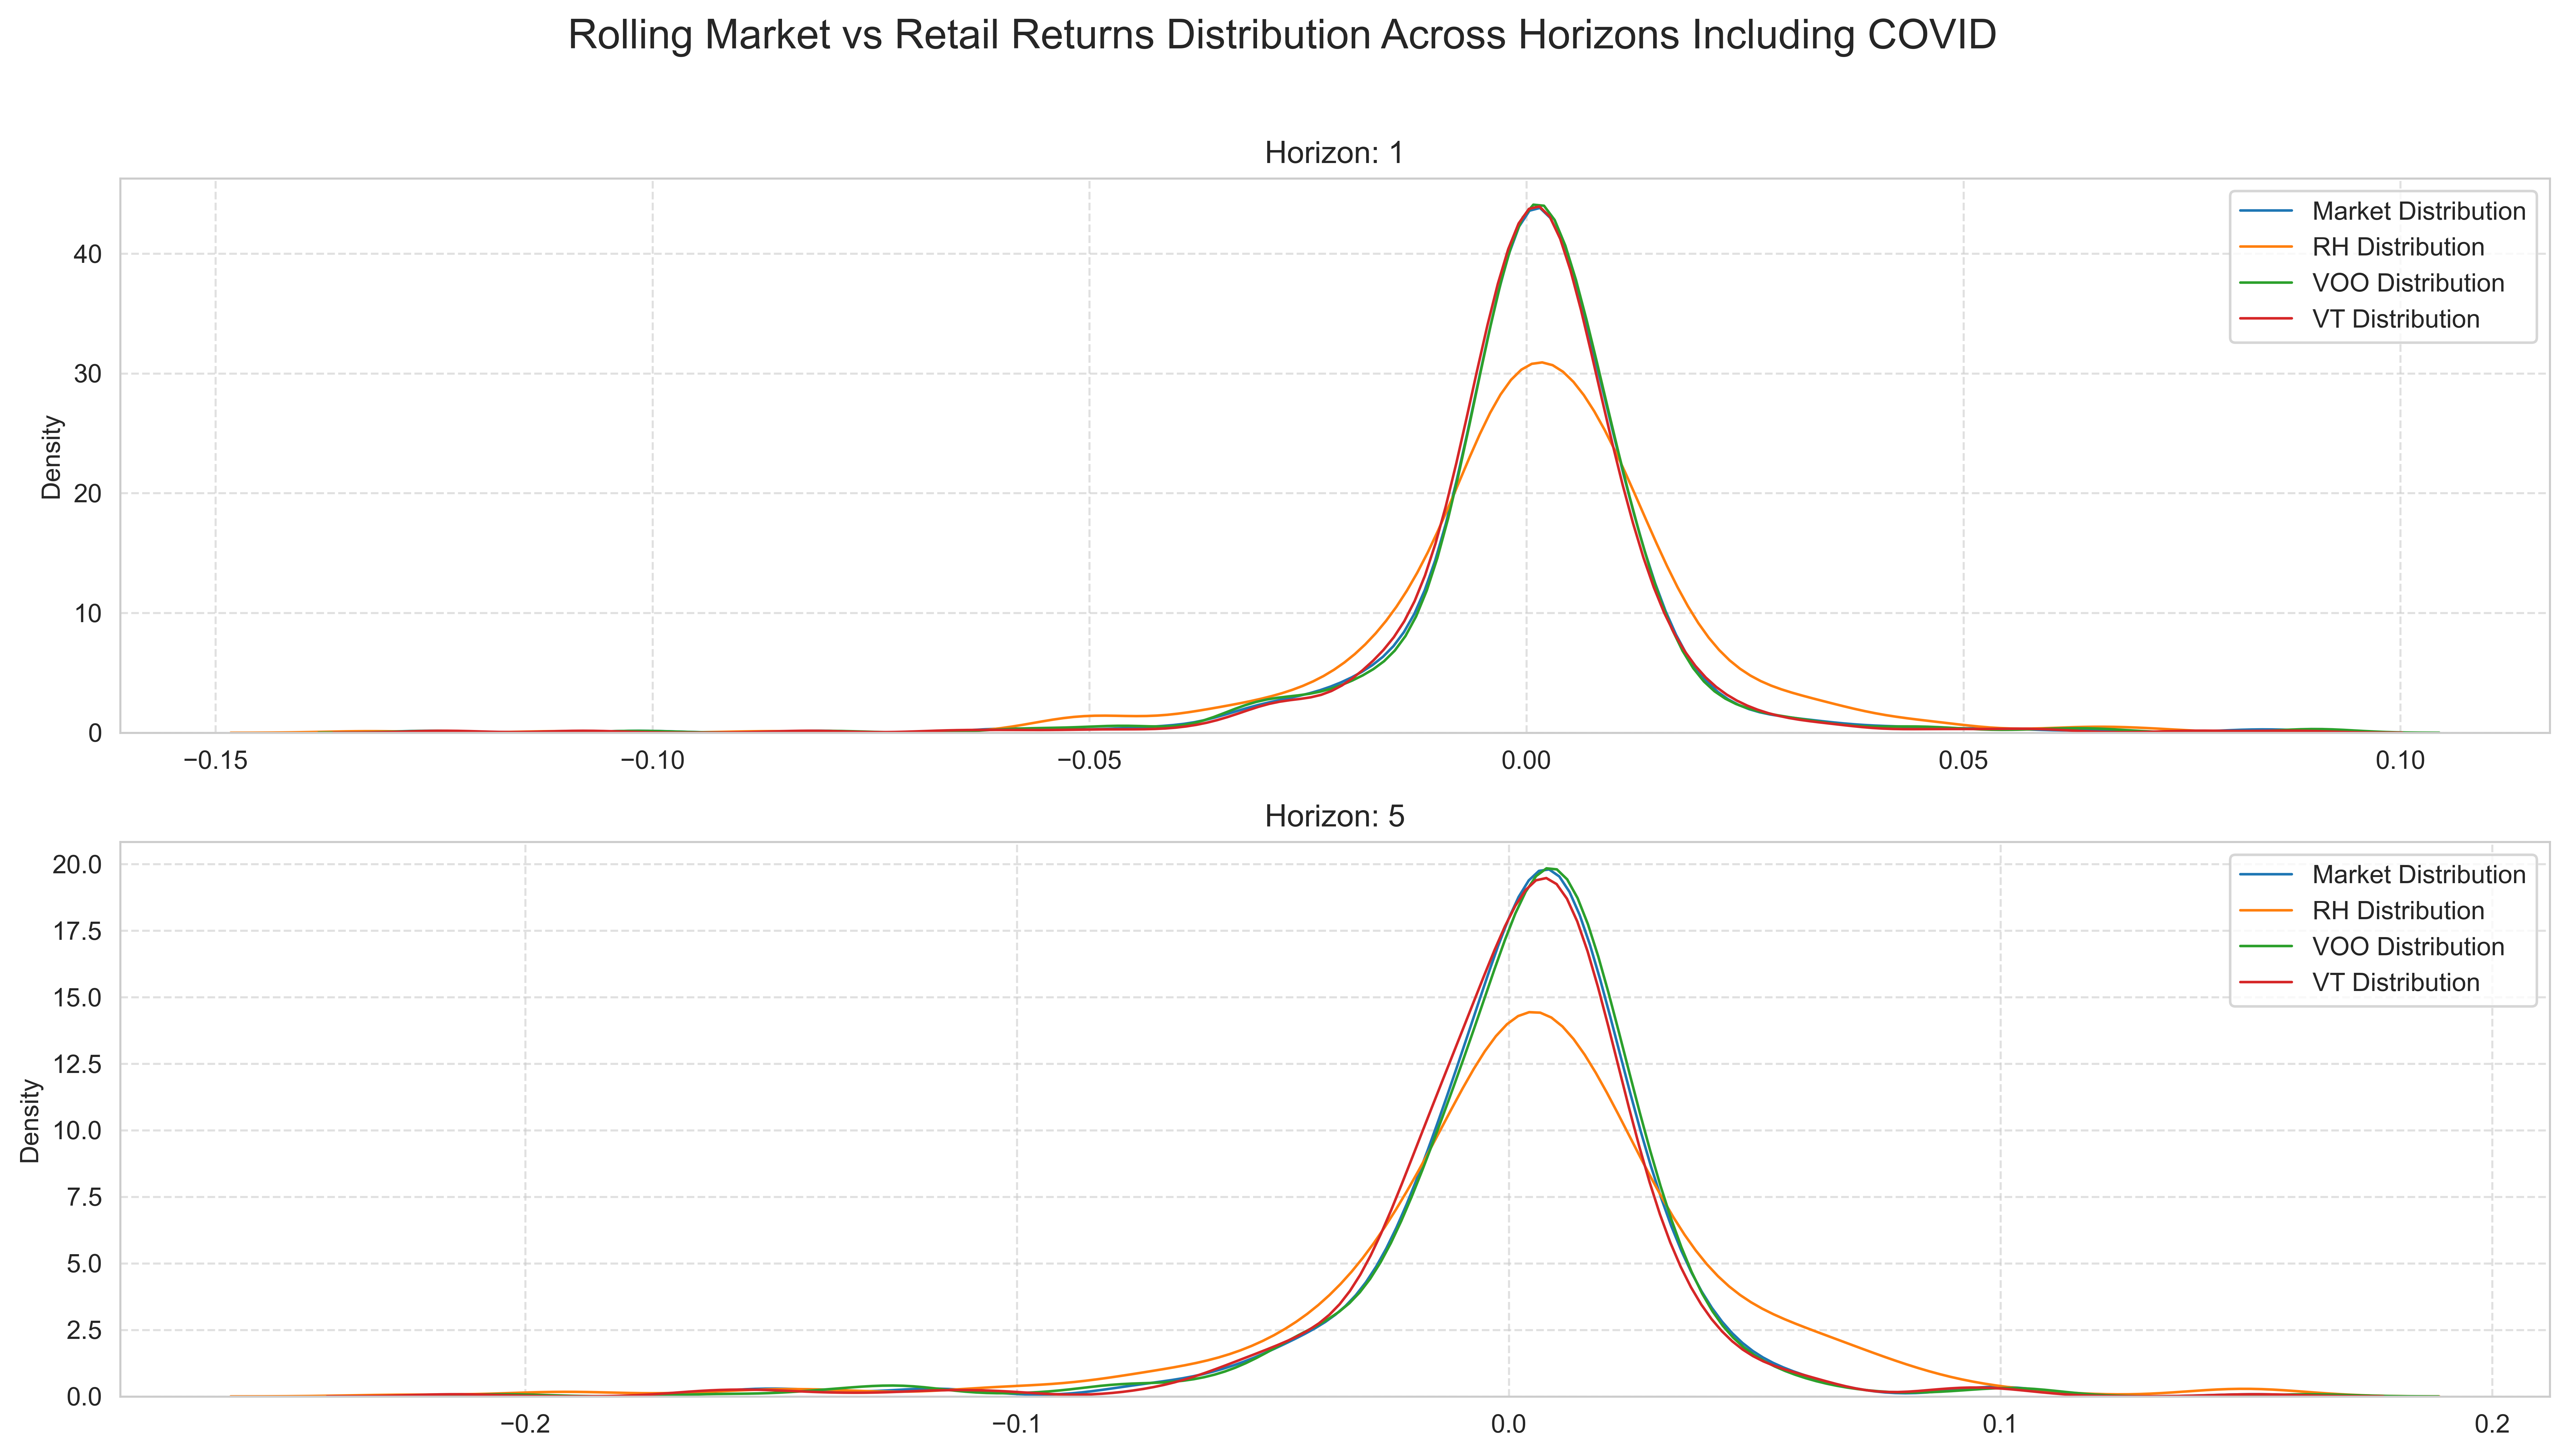
\includegraphics[width=1\linewidth]{Images/kdes_including_1_5.png}
\end{figure}

\begin{figure}[H]
    \centering
    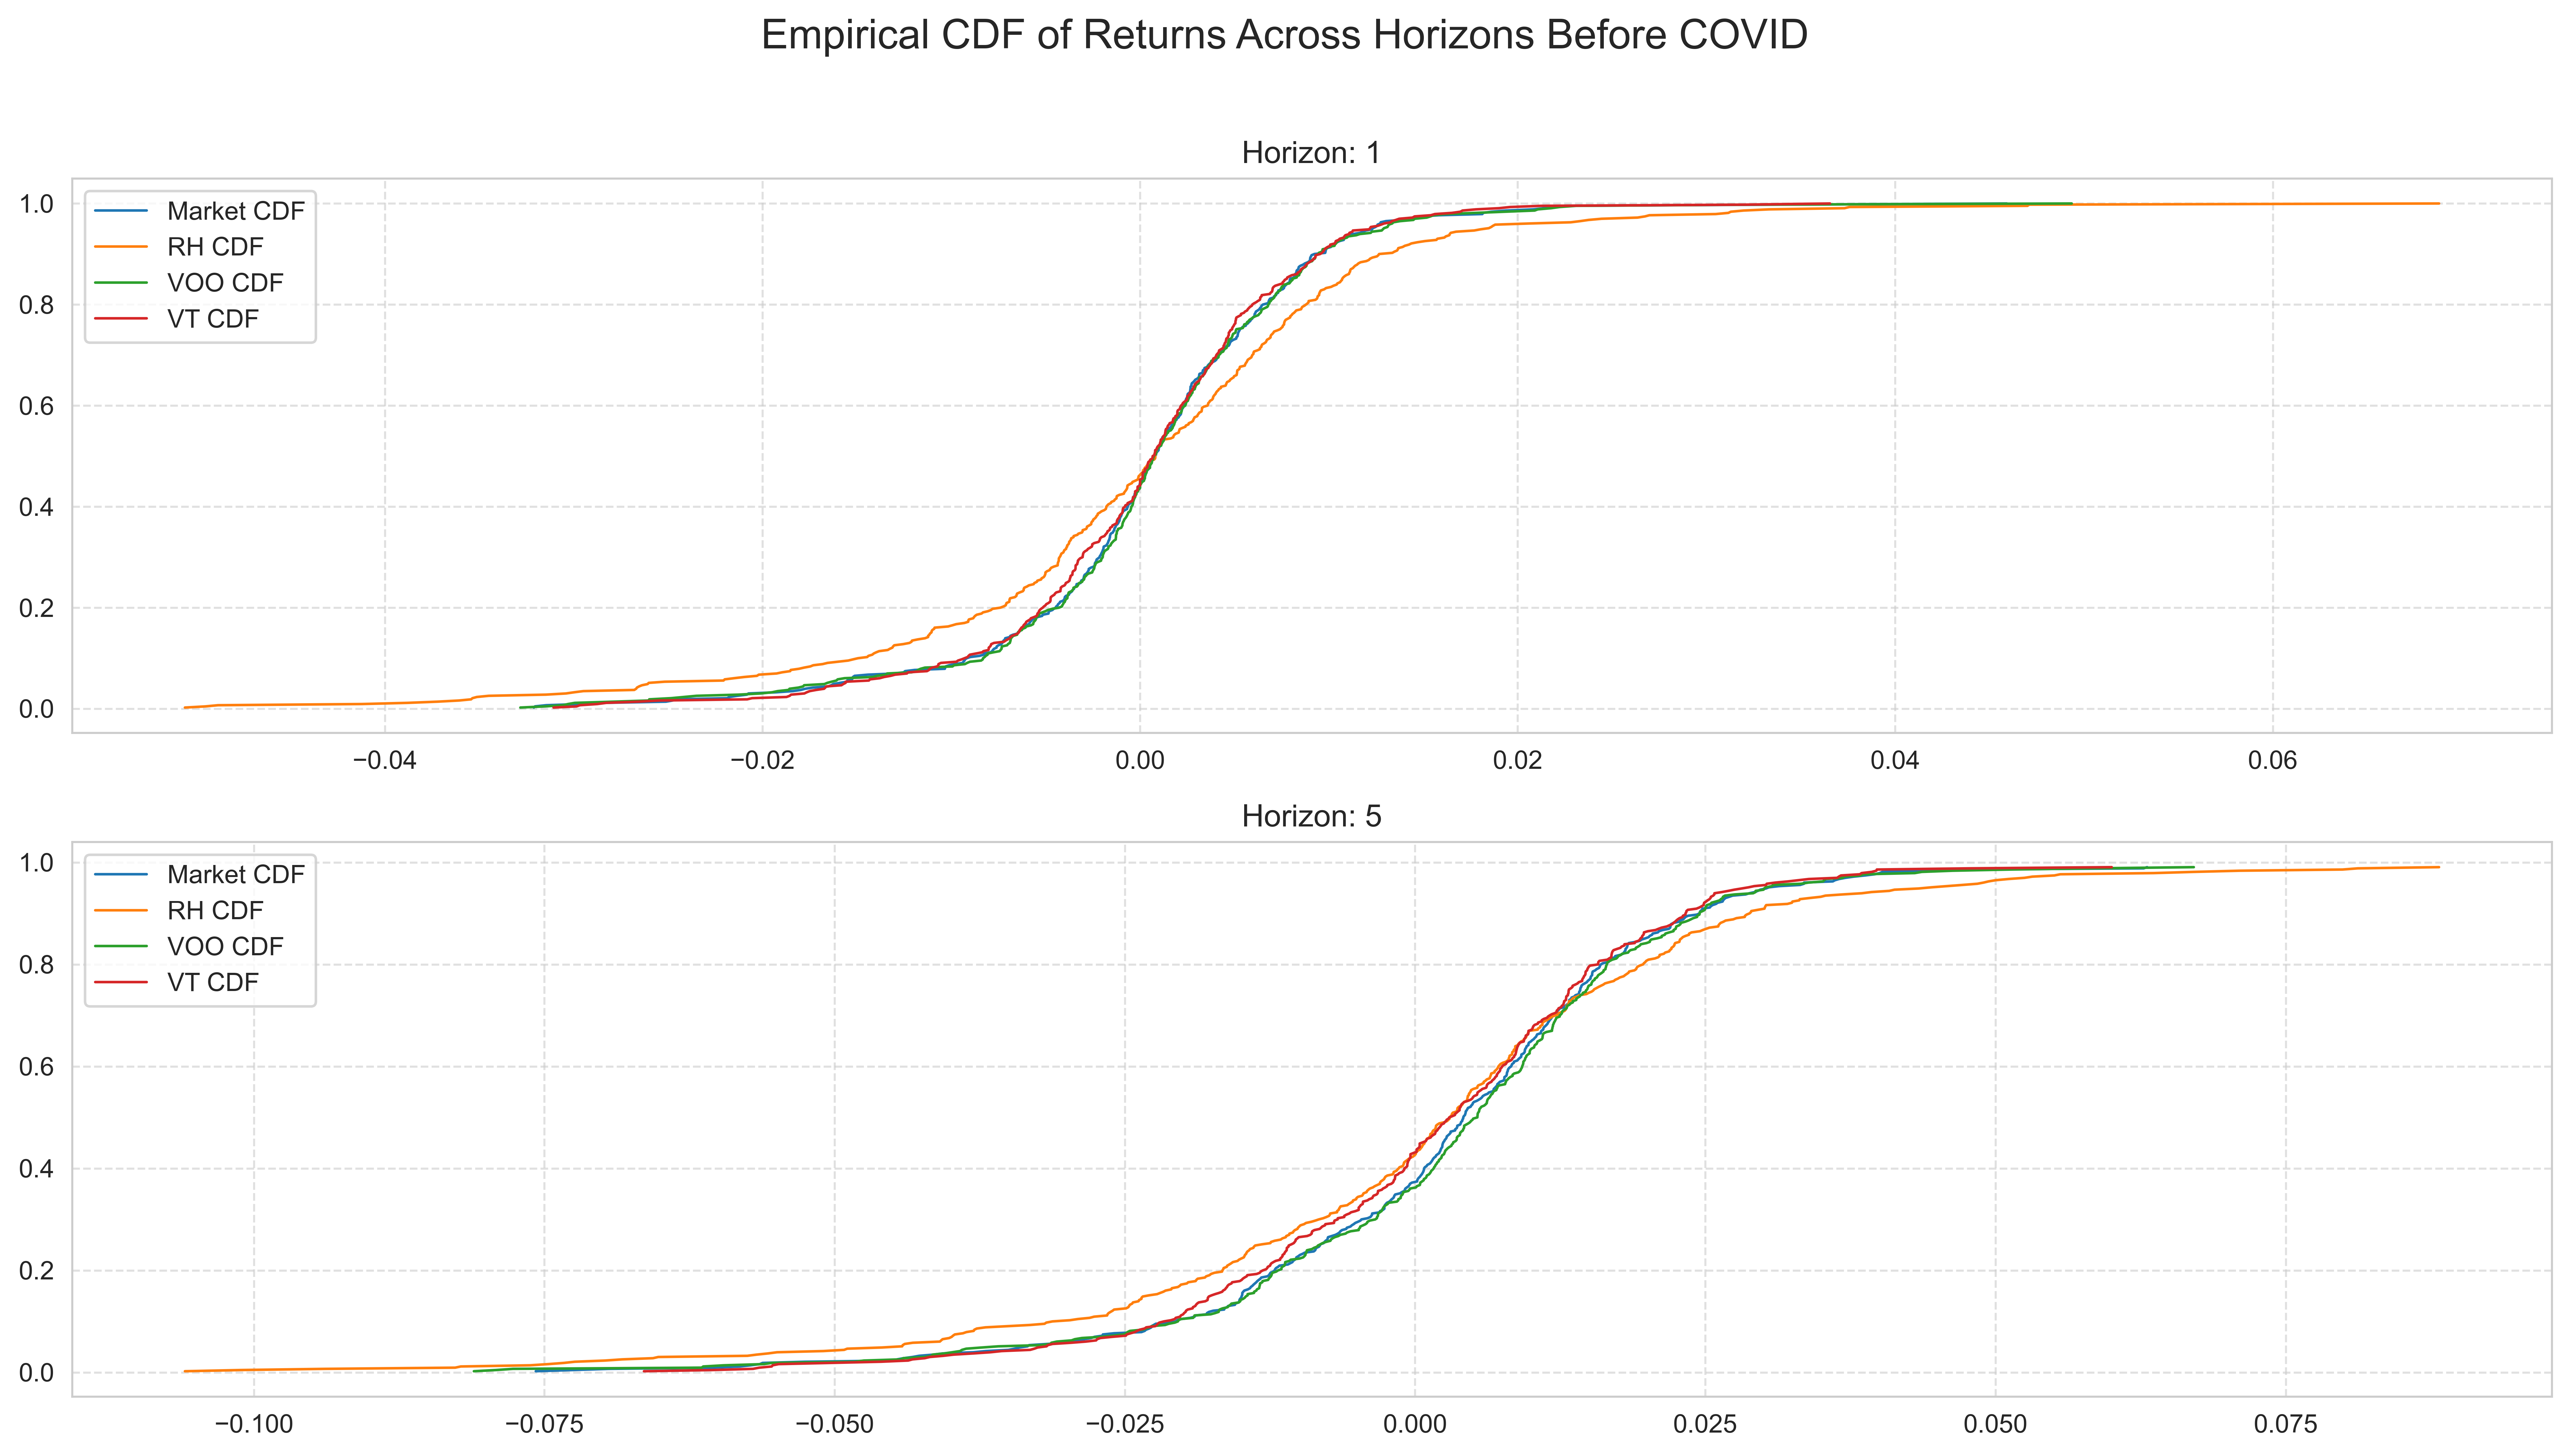
\includegraphics[width=1\linewidth]{Images/cdfs_before_1_5.png}
\end{figure}
\begin{figure}[H]
    \centering
    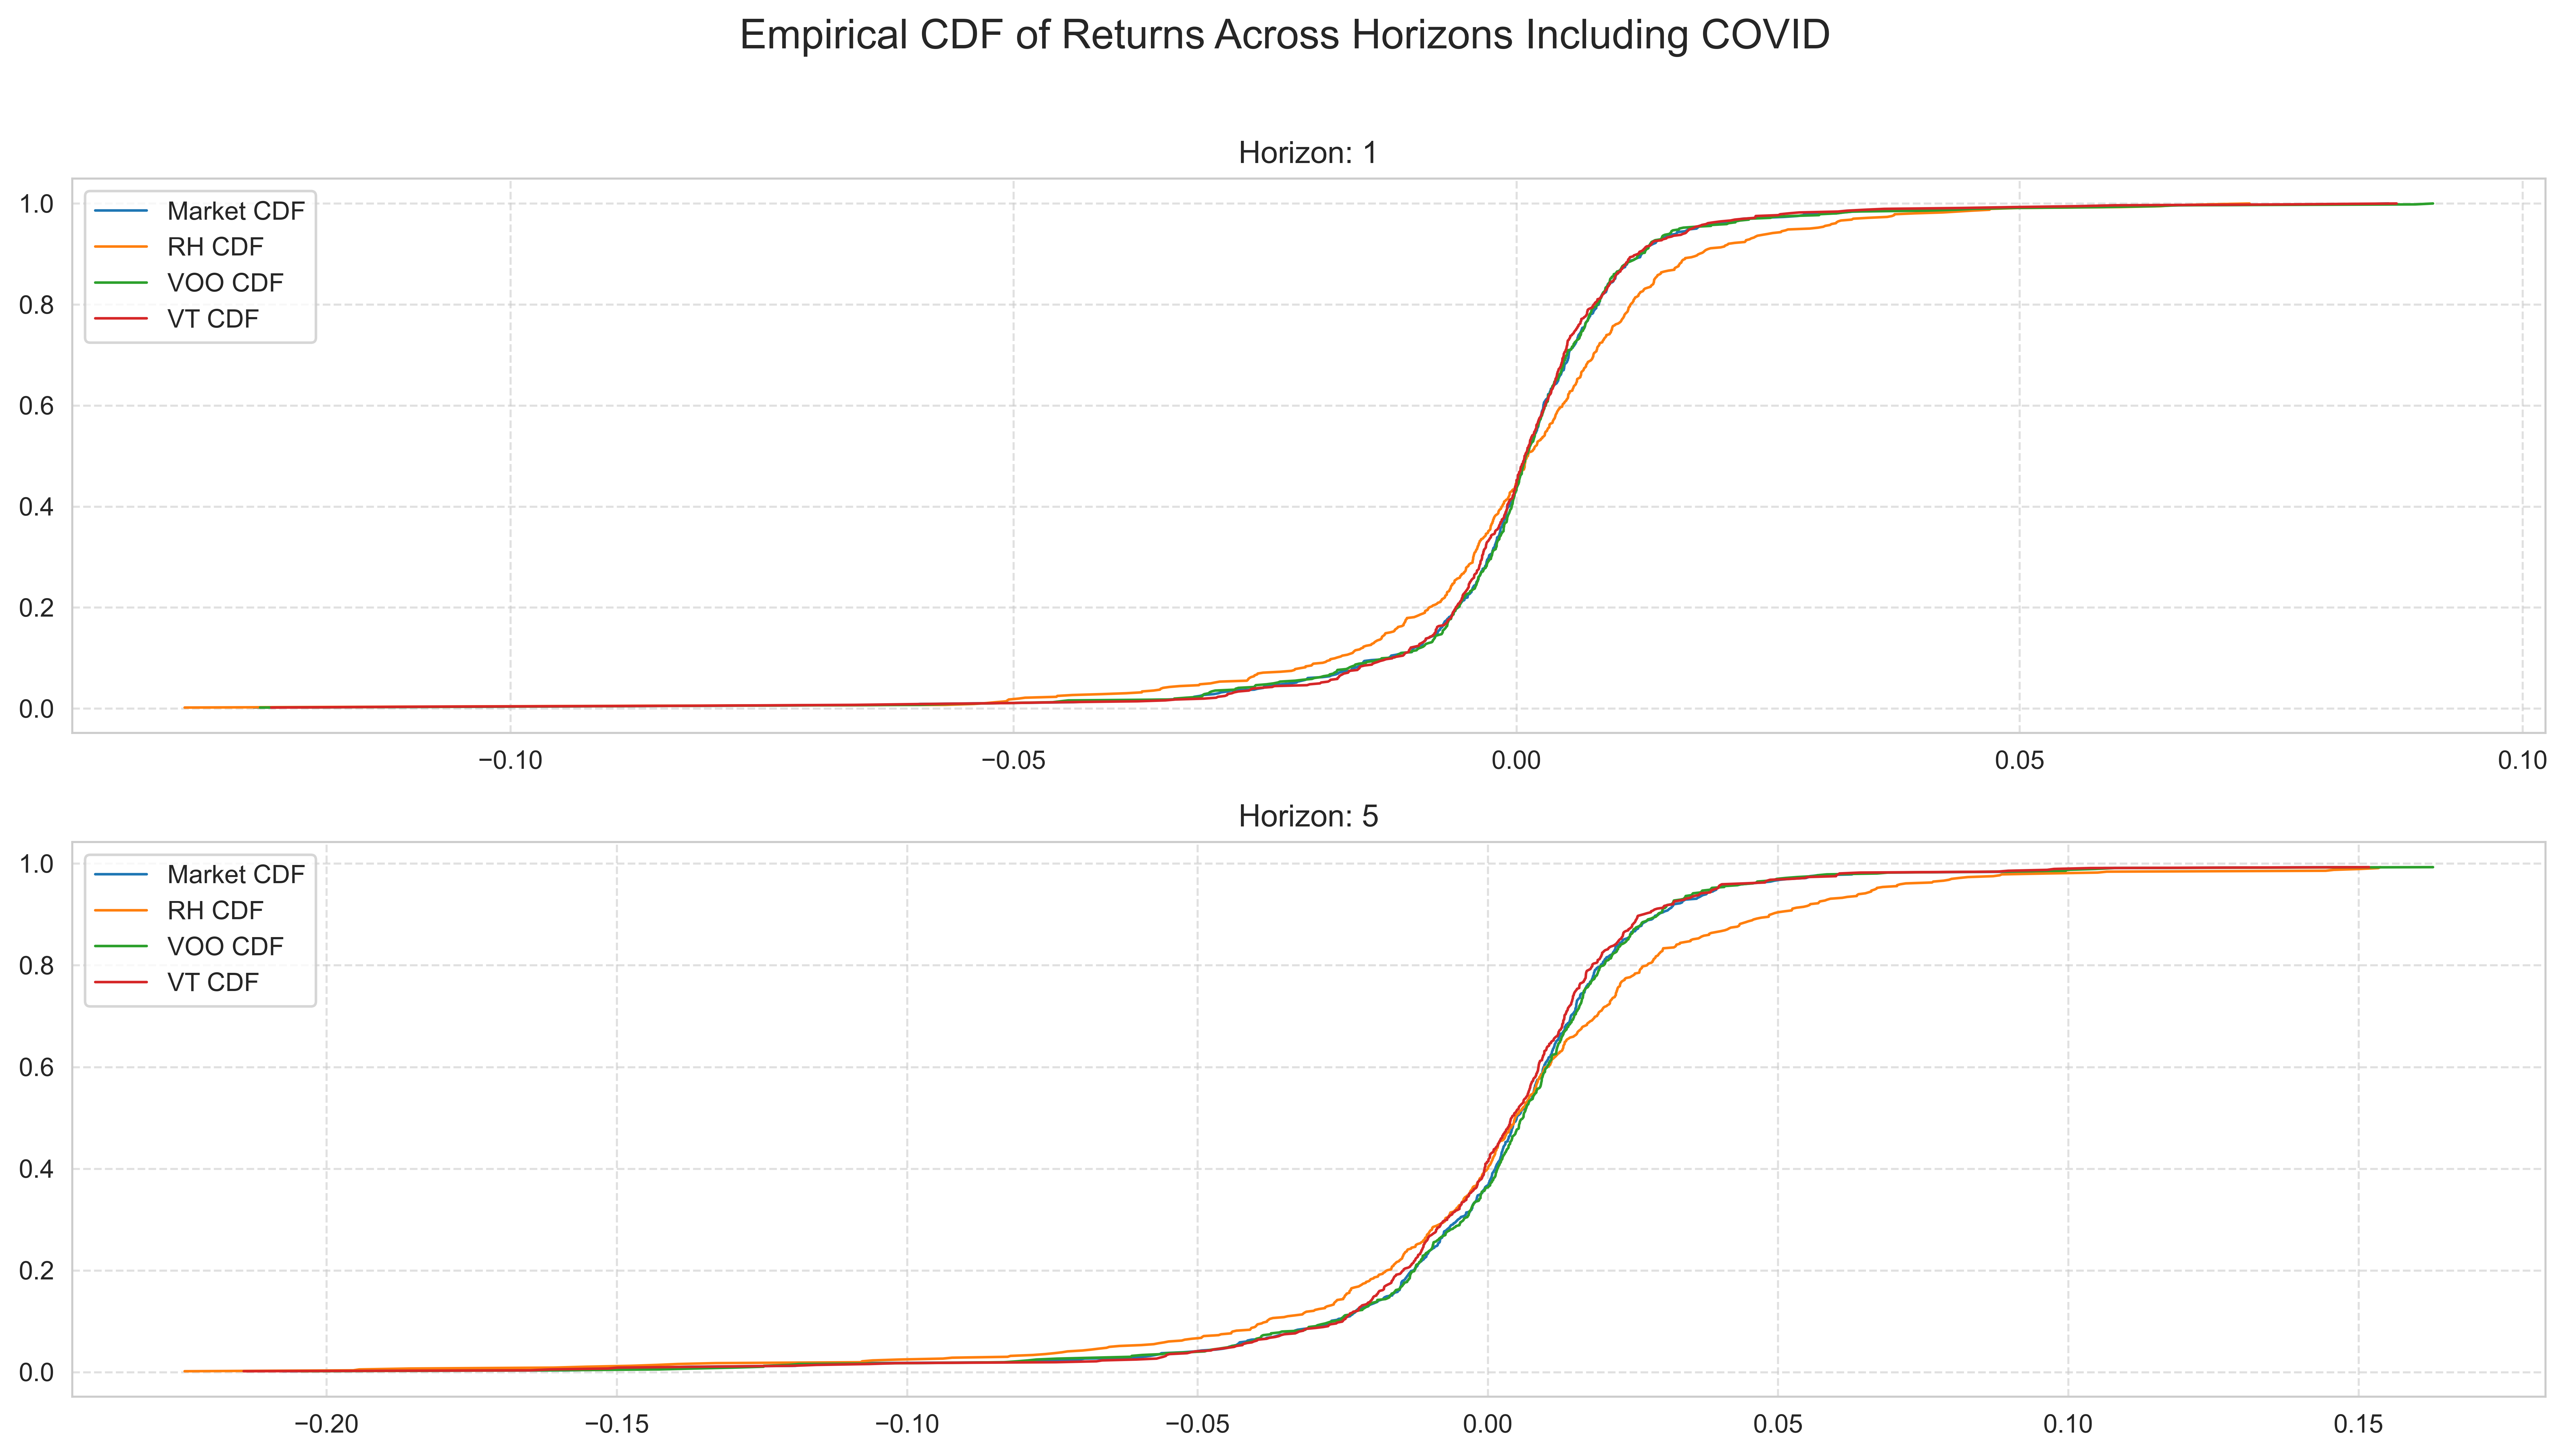
\includegraphics[width=1\linewidth]{Images/cdfs_including_1_5.png}
\end{figure}

\subsubsection{Comments}

The short-term return distribution for the RH portfolio is noticeably "flatter" (higher variance/dispersion) compared to broad market benchmarks like VOO or VT. 
This is consistent with the "buy-the-dip" behavior highlighted by \cite{Fedyk2024} and \cite{Ardia2023Fast}. 
Actively buying stocks after extreme negative returns means engaging with assets currently experiencing heightened volatility. Even if the average next-day return was positive during the sample period (as Fedyk found for 1-day holds), 
the range of potential outcomes for these stressed stocks is much wider than for the diversified market, contributing to the fatter tails and lower peak in the distribution.

    
A primary driver of the flatter distribution is likely the significant lack of diversification among individual Robinhood investors. As noted by \cite{Fedyk2024} and \cite{Welch2022}, the average user held very few stocks ($\approx3$)\footnote{They reach this measure by dividing the estimated number of active users mid august 2020 with the number of open positions}. 
Individual, concentrated portfolios inherently carry high idiosyncratic risk, leading to much greater return variance compared to diversified market indices represented by VOO/VT.
    
Stock selection tilts further contribute to the higher volatility. \cite{Welch2022} found RH investors favoured high-volume stocks, which can be associated with higher attention and volatility. 
\cite{Fedyk2024} also found no strong evidence of aversion to idiosyncratic volatility. Additionally, \cite{Ardia2023Fast} noted stronger reactions in specific sectors like energy. These preferences likely result in a basket of holdings that is intrinsically more volatile than the overall market.
